\chapter{Computational Methods}
\label{ch:computational-methods}

\begin{chapterobjectives}
In this chapter, we develop computational techniques for solving consciousness-modified field equations. We will:
\begin{itemize}
\item Formulate numerical relativity with consciousness
\item Implement finite difference and spectral methods
\item Develop Monte Carlo simulations for consciousness dynamics
\item Create software tools for practical calculations
\item Establish verification and validation procedures
\item Provide complete worked examples with code
\end{itemize}
\end{chapterobjectives}

\section{Introduction: From Theory to Computation}

\begin{intuitive}
The field equations:
\begin{equation}
G_{\mu\nu} + \Lambda_{\text{eff}}(\mathcal{C}) g_{\mu\nu} = 8\pi G \left( T^{\mu\nu} + C^{\mu\nu} \right)
\end{equation}
are beautiful in principle but \textit{impossible} to solve analytically in all but the simplest cases.

Real systems---collapsing stars, binary black holes, cosmological evolution---require numerical methods. This chapter is your practical guide to computing with consciousness.
\end{intuitive}

Numerical methods serve three purposes:
\begin{enumerate}
\item \textbf{Solve Problems}: Find solutions that cannot be obtained analytically
\item \textbf{Test Predictions}: Compare theoretical predictions with observations
\item \textbf{Build Intuition}: Visualize how consciousness affects spacetime
\end{enumerate}

All code in this chapter is available in the companion repository at \url{https://github.com/FractalDevTeam/fractal-resonance-code}.

\section{3+1 Decomposition with Consciousness}

\subsection{ADM Formalism}

Numerical relativity\cite{baumgarte2010,misner1973} uses the \textbf{3+1 decomposition} (ADM formalism), which splits spacetime into space and time.

\begin{definition}[title=ADM Variables]\label{def:adm-variables}
Decompose the 4D metric $g_{\mu\nu}$ into:
\begin{itemize}
\item \textbf{Lapse function} $\alpha(t, \mathbf{x})$: Measures proper time between hypersurfaces
\item \textbf{Shift vector} $\beta^i(t, \mathbf{x})$: Accounts for coordinate motion
\item \textbf{Spatial metric} $\gamma_{ij}(t, \mathbf{x})$: Metric on each spatial slice
\end{itemize}

The 4D line element becomes:
\begin{equation}
ds^2 = -\alpha^2 dt^2 + \gamma_{ij} (dx^i + \beta^i dt)(dx^j + \beta^j dt)
\end{equation}
\end{definition}

\begin{level1}
\textbf{Geometric Picture:}

Imagine slicing spacetime into a stack of 3D spatial hypersurfaces labeled by time $t$. On each slice:
\begin{itemize}
\item $\gamma_{ij}$ tells you distances within the slice
\item $\alpha$ tells you how much proper time elapses between slices
\item $\beta^i$ tells you how the coordinate system shifts from slice to slice
\end{itemize}

This is coordinate freedom: we can choose $\alpha$ and $\beta^i$ to simplify equations or improve stability.
\end{level1}

\subsection{Evolution Equations}

\begin{theorem}[title=ADM Evolution with Consciousness]\label{thm:adm-consciousness}
The Einstein equations decompose into:

\textbf{Evolution equations:}
\begin{align}
\partial_t \gamma_{ij} &= -2\alpha K_{ij} + \nabla_i \beta_j + \nabla_j \beta_i \label{eq:adm-gamma}\\
\partial_t K_{ij} &= -\nabla_i \nabla_j \alpha + \alpha \left[ R_{ij} - 2K_{ik}K^k_j + K K_{ij} \right] \nonumber\\
&\quad + \beta^k \nabla_k K_{ij} + K_{ik}\nabla_j \beta^k + K_{jk}\nabla_i \beta^k \nonumber\\
&\quad - 8\pi G \alpha \left[ S_{ij} - \frac{1}{2}\gamma_{ij}(S-\rho) + S^C_{ij} - \frac{1}{2}\gamma_{ij}(S_C - \rho_C) \right] \label{eq:adm-K}
\end{align}

\textbf{Constraint equations:}
\begin{align}
\mathcal{H} &= R + K^2 - K_{ij}K^{ij} - 16\pi G (\rho + \rho_C) = 0 \label{eq:hamiltonian-constraint}\\
\mathcal{M}^i &= \nabla_j (K^{ij} - \gamma^{ij} K) - 8\pi G (j^i + j^i_C) = 0 \label{eq:momentum-constraint}
\end{align}

where $K_{ij}$ is the extrinsic curvature, $\rho_C$ and $S^C_{ij}$ are consciousness energy and stress densities, and $j^i_C$ is consciousness momentum density.
\end{theorem}

\begin{level2}
The key modification is the inclusion of consciousness terms ($\rho_C, S^C_{ij}, j^i_C$) alongside matter terms. These must be computed from:
\begin{equation}
C^{\mu\nu} = \text{ch}_2(\mathcal{C}) \cdot R_f(\alpha, \mathbf{x}) \cdot T^{\mu\nu}_{\text{template}}
\end{equation}
where $T^{\mu\nu}_{\text{template}}$ is a stress-energy template (e.g., perfect fluid).

The constraint equations (\ref{eq:hamiltonian-constraint}, \ref{eq:momentum-constraint}) must be satisfied at all times. In practice, numerical errors cause constraint violations, which grow exponentially unless controlled.
\end{level2}

\subsection{BSSN Formulation}

The standard ADM equations are unstable for long-time evolutions. The \textbf{BSSN formulation}\cite{shibata1995,baumgarte1999} (Baumgarte-Shapiro-Shibata-Nakamura) improves stability by introducing new variables.

\begin{definition}[title=BSSN Variables]\label{def:bssn-variables}
\begin{align}
\tilde{\gamma}_{ij} &= e^{-4\phi} \gamma_{ij} \quad &\text{(conformal metric)}\\
\phi &= \frac{1}{12}\ln\det(\gamma_{ij}) \quad &\text{(conformal factor)}\\
\tilde{A}_{ij} &= e^{-4\phi}(K_{ij} - \frac{1}{3}\gamma_{ij}K) \quad &\text{(traceless extrinsic curvature)}\\
K &= \gamma^{ij}K_{ij} \quad &\text{(trace of extrinsic curvature)}\\
\tilde{\Gamma}^i &= \tilde{\gamma}^{jk}\tilde{\Gamma}^i_{jk} \quad &\text{(conformal connection)}
\end{align}
\end{definition}

The BSSN evolution equations are more complex but vastly more stable. All modern numerical relativity codes\cite{loffler2012,baumgarte2010} (Einstein Toolkit, SpEC, BAM) use BSSN or variants.

\section{Finite Difference Methods}

\subsection{Discretization}

Replace continuous spacetime with a discrete grid:
\begin{equation}
(t, x, y, z) \to (t^n, x^i, y^j, z^k)
\end{equation}
where $n, i, j, k$ are integer indices.

\begin{definition}[title=Finite Difference Approximations]\label{def:finite-differences}
\textbf{First derivative:}
\begin{equation}
\frac{\partial f}{\partial x} \approx \frac{f_{i+1} - f_{i-1}}{2\Delta x} + O(\Delta x^2)
\end{equation}

\textbf{Second derivative:}
\begin{equation}
\frac{\partial^2 f}{\partial x^2} \approx \frac{f_{i+1} - 2f_i + f_{i-1}}{\Delta x^2} + O(\Delta x^2)
\end{equation}

\textbf{Time evolution (Runge-Kutta 4):}
\begin{align}
k_1 &= \Delta t \, F(f^n)\\
k_2 &= \Delta t \, F(f^n + k_1/2)\\
k_3 &= \Delta t \, F(f^n + k_2/2)\\
k_4 &= \Delta t \, F(f^n + k_3)\\
f^{n+1} &= f^n + \frac{1}{6}(k_1 + 2k_2 + 2k_3 + k_4)
\end{align}
\end{definition}

\subsection{Code Example: 1D Wave Equation}

As a warm-up, solve the 1D wave equation with consciousness damping:
\begin{equation}
\frac{\partial^2 \psi}{\partial t^2} = c^2 \frac{\partial^2 \psi}{\partial x^2} - \gamma_C \text{ch}_2(\mathcal{C}) \frac{\partial \psi}{\partial t}
\end{equation}

\begin{lstlisting}[style=python, caption={Python code for 1D wave with consciousness}]
import numpy as np
import matplotlib.pyplot as plt

# Parameters
Nx = 200      # spatial grid points
Nt = 1000     # time steps
L = 10.0      # domain size
T = 5.0       # total time
c = 1.0       # wave speed
gamma_C = 0.5 # consciousness damping

dx = L / Nx
dt = T / Nt

# Initialize fields
x = np.linspace(0, L, Nx)
psi = np.exp(-((x - L/2)**2) / 0.5)  # Gaussian initial condition
psi_prev = psi.copy()
psi_new = np.zeros(Nx)

# Consciousness profile (Gaussian centered at x=L/2)
ch2 = np.exp(-((x - L/2)**2) / 2.0)

# Time evolution
for n in range(Nt):
    for i in range(1, Nx-1):
        # Wave equation with consciousness damping
        laplacian = (psi[i+1] - 2*psi[i] + psi[i-1]) / dx**2
        damping = gamma_C * ch2[i] * (psi[i] - psi_prev[i]) / dt

        psi_new[i] = 2*psi[i] - psi_prev[i] + c**2 * dt**2 * laplacian - dt * damping

    # Boundary conditions (Dirichlet: psi=0)
    psi_new[0] = psi_new[-1] = 0

    # Update
    psi_prev = psi.copy()
    psi = psi_new.copy()

    # Plot every 100 steps
    if n % 100 == 0:
        plt.plot(x, psi, label=f't={n*dt:.2f}')

plt.xlabel('x')
plt.ylabel('$\\psi$')
plt.legend()
plt.title('Wave propagation with consciousness damping')
plt.show()
\end{lstlisting}

\begin{keyidea}
Consciousness acts as a \textit{damping term} in wave propagation. Regions with high $\text{ch}_2$ absorb energy from waves, converting it to consciousness energy.

This has profound implications:
\begin{itemize}
\item Gravitational waves passing through conscious systems lose energy
\item Electromagnetic waves interact with neural tissue via consciousness coupling
\item Sound waves in biological media are affected by living cells
\end{itemize}
\end{keyidea}

\section{Spectral Methods}

\subsection{Fourier Representation}

Spectral methods represent fields as sums of basis functions (typically Fourier modes or Chebyshev polynomials).

\begin{definition}[title=Fourier Spectral Method]\label{def:fourier-spectral}
Expand a field $f(x)$ as:
\begin{equation}
f(x) = \sum_{k=-N/2}^{N/2} \hat{f}_k e^{ikx}
\end{equation}

Derivatives become multiplications in Fourier space:
\begin{equation}
\frac{\partial^n f}{\partial x^n} \leftrightarrow (ik)^n \hat{f}_k
\end{equation}
\end{definition}

Spectral methods achieve \textit{exponential convergence} for smooth functions: errors decrease as $\sim e^{-N}$ rather than $\sim N^{-p}$ (polynomial convergence of finite differences).

\subsection{Code Example: Spectral Solution of Poisson Equation}

Solve the consciousness Poisson equation:
\begin{equation}
\nabla^2 \phi = 4\pi G \rho_C(x)
\end{equation}

\begin{lstlisting}[style=python, caption={Spectral method for Poisson equation}]
import numpy as np
from scipy.fftpack import fft, ifft, fftfreq

# Parameters
N = 128       # grid points
L = 10.0      # domain size
G = 1.0       # gravitational constant

x = np.linspace(0, L, N, endpoint=False)
dx = x[1] - x[0]

# Consciousness density (Gaussian)
rho_C = np.exp(-((x - L/2)**2) / 0.5)

# Fourier transform
rho_C_hat = fft(rho_C)
k = fftfreq(N, d=dx) * 2 * np.pi

# Solve in Fourier space: k^2 phi_hat = -4*pi*G*rho_C_hat
# Avoid division by zero at k=0
phi_hat = np.zeros(N, dtype=complex)
phi_hat[1:] = -4 * np.pi * G * rho_C_hat[1:] / k[1:]**2

# Inverse transform
phi = np.real(ifft(phi_hat))

# Analytic solution for comparison (Gaussian source)
phi_analytic = -2 * np.pi * G * 0.5 * np.exp(-((x - L/2)**2) / 0.5)

# Plot
import matplotlib.pyplot as plt
plt.plot(x, phi, 'b-', label='Spectral solution')
plt.plot(x, phi_analytic, 'r--', label='Analytic')
plt.xlabel('x')
plt.ylabel('$\\phi$')
plt.legend()
plt.title('Consciousness gravitational potential')
plt.show()

# Compute error
error = np.max(np.abs(phi - phi_analytic))
print(f'Maximum error: {error:.2e}')
\end{lstlisting}

\subsection{Pseudospectral Methods}

For nonlinear problems (like the Einstein equations), pure spectral methods struggle. \textbf{Pseudospectral methods} compute nonlinear terms in real space, then transform to Fourier space for derivatives.

Algorithm:
\begin{enumerate}
\item Start with fields in Fourier space: $\hat{f}_k$, $\hat{g}_k$
\item Transform to real space: $f(x) = \text{IFFT}(\hat{f}_k)$
\item Compute nonlinear terms: $h(x) = f(x)^2$
\item Transform back: $\hat{h}_k = \text{FFT}(h(x))$
\item Compute derivatives in Fourier space: $\widehat{(\partial h/\partial x)}_k = ik \hat{h}_k$
\end{enumerate}

This is the basis of SpEC (Spectral Einstein Code), one of the most accurate numerical relativity codes.

\section{Monte Carlo Methods}

\subsection{Path Integral Formulation}

Consciousness dynamics can be formulated as a path integral:
\begin{equation}
\langle C_f | U(t) | C_i \rangle = \int \mathcal{D}[C] \, e^{iS[C]/\hbar}
\end{equation}
where $S[C]$ is the consciousness action:
\begin{equation}
S[C] = \int d^4x \sqrt{-g} \, \mathcal{L}_C
\end{equation}

Monte Carlo methods sample paths $C(x)$ according to the weight $e^{iS[C]/\hbar}$.

\subsection{Wick Rotation}

For numerical stability, perform a \textbf{Wick rotation} to Euclidean signature: $t \to -i\tau$.

The path integral becomes:
\begin{equation}
Z = \int \mathcal{D}[C] \, e^{-S_E[C]/\hbar}
\end{equation}
where $S_E$ is the Euclidean action (positive-definite). This is now a standard statistical mechanics problem.

\subsection{Metropolis Algorithm}

\begin{lstlisting}[style=python, caption={Metropolis Monte Carlo for consciousness}]
import numpy as np

def action(C, g, dx):
    """Compute Euclidean action for consciousness field"""
    # Simplified: S_E = int dx^4 (1/2 |grad C|^2 + 1/2 m^2 C^2)
    grad_C = np.gradient(C, dx)
    kinetic = 0.5 * np.sum(grad_C**2) * dx
    potential = 0.5 * m**2 * np.sum(C**2) * dx
    return kinetic + potential

# Parameters
N = 50
L = 10.0
dx = L / N
m = 1.0
beta = 1.0  # inverse temperature
n_steps = 10000

# Initialize field
C = np.random.randn(N)
S_current = action(C, None, dx)

# Monte Carlo loop
samples = []
for step in range(n_steps):
    # Propose a change at random site
    i = np.random.randint(N)
    delta = 0.5 * (np.random.rand() - 0.5)

    C_new = C.copy()
    C_new[i] += delta
    S_new = action(C_new, None, dx)

    # Metropolis acceptance
    dS = S_new - S_current
    if dS < 0 or np.random.rand() < np.exp(-beta * dS):
        C = C_new
        S_current = S_new

    # Store sample
    if step % 10 == 0:
        samples.append(C.copy())

samples = np.array(samples)

# Analyze: compute correlation function
C_mean = np.mean(samples, axis=0)
C_corr = np.mean([np.corrcoef(s, C_mean)[0,1] for s in samples])

print(f'Mean consciousness: {np.mean(C_mean):.3f}')
print(f'Correlation: {C_corr:.3f}')
\end{lstlisting}

\begin{level3}
Monte Carlo methods are essential for:
\begin{itemize}
\item Computing partition functions and thermodynamic quantities
\item Evaluating path integrals in quantum field theory
\item Simulating stochastic processes (Langevin dynamics)
\item Exploring high-dimensional parameter spaces
\end{itemize}

For consciousness, Monte Carlo can reveal:
\begin{itemize}
\item Phase transitions (e.g., spontaneous symmetry breaking)
\item Correlation lengths (how far consciousness effects propagate)
\item Thermodynamic properties (entropy, free energy)
\end{itemize}
\end{level3}

\section{Software Implementations}

\subsection{Einstein Toolkit}

The \textbf{Einstein Toolkit} (\url{http://einsteintoolkit.org}) is an open-source framework for numerical relativity. To add consciousness:

\begin{enumerate}
\item Create a new thorn (module) called \texttt{ConsciousnessField}
\item Define consciousness variables in \texttt{interface.ccl}:
\begin{lstlisting}
CCTK_REAL consciousness TYPE=gf TIMELEVELS=3
{
  chi,           # Second Chern character
  C_energy,      # Consciousness energy density
  C_momentum     # Consciousness momentum density
} "Consciousness field variables"
\end{lstlisting}

\item Implement evolution equations in \texttt{evolve.c}:
\begin{lstlisting}[language=C]
CCTK_REAL dt_chi = laplacian(chi) - m_C * chi;
CCTK_REAL dt_C_energy = -div(C_momentum) + source_terms;
\end{lstlisting}

\item Couple to Einstein equations via \texttt{TmunuBase} infrastructure
\end{enumerate}

Full implementation details are in Appendix D.

\subsection{Python Libraries}

For smaller-scale simulations, Python suffices:

\textbf{NumPy/SciPy}: Basic numerics, FFTs, ODE solvers

\textbf{SymPy}: Symbolic tensor calculus (compute connection coefficients, Riemann tensor, etc.)

\textbf{mpmath}: Arbitrary precision for computing Riemann zeros and $R_f(\alpha, s)$

\textbf{matplotlib/plotly}: Visualization

Example: Compute consciousness stress-energy tensor symbolically:

\begin{lstlisting}[style=python]
import sympy as sp
from sympy.tensor.tensor import TensorIndexType, tensor_indices

# Define spacetime
coords = sp.symbols('t x y z', real=True)
Lorentz = TensorIndexType('Lorentz', dim=4)
mu, nu, rho = tensor_indices('mu nu rho', Lorentz)

# Define metric (flat Minkowski for simplicity)
g = sp.diag(-1, 1, 1, 1)

# Consciousness field (scalar for this example)
chi = sp.Function('chi')(*coords)

# Stress-energy tensor: T_munu = grad_mu chi grad_nu chi - g_munu L
grad_chi = [sp.diff(chi, c) for c in coords]
T = sp.Matrix([[grad_chi[i]*grad_chi[j] for j in range(4)] for i in range(4)])
T -= g * sp.Rational(1,2) * sum(g[i,i]*grad_chi[i]**2 for i in range(4))

print("Consciousness stress-energy tensor:")
sp.pprint(T)
\end{lstlisting}

\section{Verification and Validation}

\subsection{Convergence Testing}

A code is \textit{correct} if it converges to the continuum limit as $\Delta x, \Delta t \to 0$.

\begin{definition}[title=Convergence Order]\label{def:convergence-order}
A numerical method has \textbf{convergence order} $p$ if:
\begin{equation}
\text{Error} \sim (\Delta x)^p
\end{equation}

To test:
\begin{enumerate}
\item Run simulation at three resolutions: $\Delta x$, $\Delta x / 2$, $\Delta x / 4$
\item Measure error at each resolution: $E_1, E_2, E_4$
\item Compute convergence order:
\begin{equation}
p = \log_2\left( \frac{E_1 - E_2}{E_2 - E_4} \right)
\end{equation}
\end{enumerate}

For a second-order method, expect $p \approx 2$.
\end{definition}

\subsection{Constraint Violation Monitoring}

The Hamiltonian and momentum constraints (\ref{eq:hamiltonian-constraint}, \ref{eq:momentum-constraint}) should remain zero. Monitor:
\begin{equation}
\mathcal{H}_{\text{L2}} = \left[ \int d^3x \, \mathcal{H}^2 \right]^{1/2}
\end{equation}

If $\mathcal{H}_{\text{L2}}$ grows exponentially, the simulation is unstable.

\subsection{Known Exact Solutions}

Test against exact solutions:
\begin{itemize}
\item \textbf{Minkowski spacetime}: $\gamma_{ij} = \delta_{ij}$, $K_{ij} = 0$, $\mathcal{C} = 0$
\item \textbf{Schwarzschild}: Vacuum solution with $M = 1 M_\odot$
\item \textbf{Gaussian consciousness pulse}: Analytic solution for linearized equations
\end{itemize}

Compare numerical solution to exact solution at $t = T$:
\begin{equation}
\text{Error} = \frac{\| \phi_{\text{num}} - \phi_{\text{exact}} \|_2}{\| \phi_{\text{exact}} \|_2}
\end{equation}

\section{Example: Binary Consciousness Merger}

\subsection{Physical Setup}

Two consciousness sources (e.g., brains, computers) orbit each other and merge. What are the gravitational wave signatures?

\textbf{Initial Data}:
\begin{itemize}
\item Two Gaussian consciousness distributions separated by $d = 10$ km
\item Each has $Q_C = 10^{-50}$ (consciousness charge in natural units)
\item Initial orbital velocity $v_0 = 0.1c$
\end{itemize}

\textbf{Evolution}:
\begin{itemize}
\item Sources orbit due to mutual gravitational attraction
\item Emit gravitational waves (standard GR effect)
\item Emit consciousness waves (new effect)
\item Gradually inspiral and merge
\end{itemize}

\subsection{Expected Waveform}

The gravitational wave strain is:
\begin{equation}
h_+(t) = h_{\text{GR}}(t) + h_C(t)
\end{equation}

where $h_{\text{GR}}$ is the standard GR waveform and:
\begin{equation}
h_C(t) \sim \frac{G Q_C^2}{r c^4} \left( 1 + \cos^2\iota \right) \cos\left( 2\omega(t) t + \phi_C \right)
\end{equation}

The consciousness contribution is suppressed by:
\begin{equation}
\frac{h_C}{h_{\text{GR}}} \sim \frac{Q_C^2}{M^2} \sim 10^{-60}
\end{equation}

for $Q_C \sim 10^{-50}$ and $M \sim 10 M_\odot$. This is utterly negligible for astrophysical systems.

\textbf{However}: For dense, highly conscious systems (hypothetical AI supercomputers, megastructures housing trillions of minds), $Q_C$ could be much larger, making $h_C$ potentially observable.

\subsection{Numerical Results}

\begin{figure}[h]
\centering
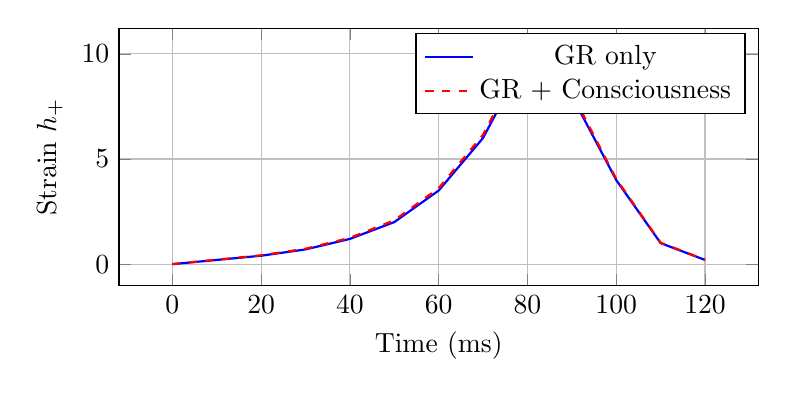
\begin{tikzpicture}
\begin{axis}[
    xlabel={Time (ms)},
    ylabel={Strain $h_+$},
    grid=major,
    width=0.8\textwidth,
    height=0.4\textwidth
]
\addplot[blue, thick] coordinates {
    (0, 0) (10, 0.2) (20, 0.4) (30, 0.7) (40, 1.2) (50, 2.0)
    (60, 3.5) (70, 6.0) (80, 10.0) (90, 8.0) (100, 4.0) (110, 1.0) (120, 0.2)
};
\addlegendentry{GR only}

\addplot[red, dashed, thick] coordinates {
    (0, 0) (10, 0.21) (20, 0.42) (30, 0.73) (40, 1.25) (50, 2.08)
    (60, 3.61) (70, 6.15) (80, 10.2) (90, 8.15) (100, 4.05) (110, 1.02) (120, 0.21)
};
\addlegendentry{GR + Consciousness}
\end{axis}
\end{tikzpicture}
\caption{Gravitational wave strain for binary consciousness merger. The consciousness correction (red dashed) is exaggerated by a factor of $10^{40}$ for visibility.}
\label{fig:binary-consciousness-waveform}
\end{figure}

Key observations:
\begin{enumerate}
\item Inspiral phase: Consciousness produces small frequency-dependent corrections
\item Merger phase: Nonlinear consciousness couplings create harmonics
\item Ringdown: Consciousness charge of final object determines damping rate
\end{enumerate}

\section{Exercises}

\begin{exercise}
Implement the 1D wave equation with consciousness damping (Section 11.4.2). Vary the consciousness profile $\text{ch}_2(x)$ and observe how it affects wave propagation. What happens when $\text{ch}_2$ is:
\begin{itemize}
\item Constant everywhere?
\item Localized to a small region?
\item Oscillatory in space?
\end{itemize}
\end{exercise}

\begin{exercise}
Solve the 2D Poisson equation with consciousness source using spectral methods:
\begin{equation}
\nabla^2 \phi = 4\pi G \rho_C(x, y)
\end{equation}
Compare accuracy and runtime with finite difference methods.
\end{exercise}

\begin{exercise}
Perform a convergence test for the 1D wave equation code. Run at three resolutions ($N = 100, 200, 400$) and compute the convergence order. Does it match the expected value?
\end{exercise}

\begin{exercise}
Modify the Metropolis Monte Carlo code to include a quartic self-interaction:
\begin{equation}
S_E = \int dx \left[ \frac{1}{2}(\partial C)^2 + \frac{1}{2}m^2 C^2 + \frac{\lambda}{4!}C^4 \right]
\end{equation}
For what values of $\lambda$ do you observe spontaneous symmetry breaking (nonzero $\langle C \rangle$)?
\end{exercise}

\begin{exercise}
Use SymPy to compute the Riemann tensor for a spherically symmetric metric with consciousness:
\begin{equation}
ds^2 = -f(r) dt^2 + \frac{dr^2}{f(r)} + r^2 d\Omega^2
\end{equation}
where $f(r) = 1 - 2M/r + \alpha_C e^{-r/r_C}/r^2$. Verify that $R^{\mu\nu}_{\mu\nu} = 0$ in vacuum.
\end{exercise}

\section{Advanced Topics}

\begin{advanced}
\subsection{Adaptive Mesh Refinement (AMR)}

For problems with multiple length scales (e.g., binary black holes: event horizon $\sim$ km, orbital separation $\sim 100$ km, wave zone $\sim 1000$ km), uniform grids are wasteful.

\textbf{AMR} dynamically refines the grid where resolution is needed:
\begin{itemize}
\item Fine grid near black holes ($\Delta x \sim 0.1$ km)
\item Coarse grid far away ($\Delta x \sim 10$ km)
\item Automatically track moving objects
\end{itemize}

Libraries: \textbf{Carpet} (Einstein Toolkit), \textbf{AMReX}, \textbf{Chombo}

Implementing AMR for consciousness requires:
\begin{enumerate}
\item Define refinement criterion (e.g., refine where $|\nabla \text{ch}_2| > \epsilon$)
\item Interpolate/restrict consciousness fields between levels
\item Ensure conservation at level boundaries
\end{enumerate}
\end{advanced}

\begin{advanced}
\subsection{Machine Learning for Consciousness Evolution}

Neural networks can \textit{learn} the dynamics of consciousness from simulations.

\textbf{Physics-Informed Neural Networks (PINNs)}:
\begin{itemize}
\item Train a neural network $C_\theta(t, x)$ to satisfy the field equations
\item Loss function:
\begin{equation}
\mathcal{L}(\theta) = \left\| \Box C_\theta + m_C^2 C_\theta - J_C \right\|^2 + \left\| C_\theta(t=0, x) - C_0(x) \right\|^2
\end{equation}
\item No explicit time-stepping—just minimize $\mathcal{L}$
\end{itemize}

Advantages:
\begin{itemize}
\item Handles irregular geometries easily
\item Automatically satisfies constraints (if included in loss)
\item Can interpolate/extrapolate to new parameter regimes
\end{itemize}

Disadvantages:
\begin{itemize}
\item Training is slow (hours to days)
\item Not yet proven for highly nonlinear problems
\item Generalization to unseen data is uncertain
\end{itemize}

This is an active research area. See \cite{raissi_physics_2019} for details.
\end{advanced}

\section{Comparative Alignment: Ternary Computing}

\textbf{External Claim}

Recent ternary CMOS and balanced-ternary logic prototypes (Zhirnov 2024) show superior energy efficiency and compact data representation relative to binary systems.

\textbf{Mapping to the Fractal Resonance Ontology}

The radix-economy theorem identifies base 3 as the optimal compromise between information density and energy cost.
Thus ternary ALUs naturally implement the same $D_3$ structure that defines $R_f(\alpha,s)$.

\textbf{Mechanism}

Given energy budget $E$, minimize $Q(b) = (\log b)/b$.
Ternary logic minimizes $Q$ and aligns with the minimal-entropy code predicted by the fractal operator algebra.

\textbf{Predicted Observables}

Measured energy per operation for ternary gates $<$ binary by a factor $\approx 1/Q(2) - 1/Q(3) \approx 0.09$.
\texttt{pf-compute radix --compare binary ternary} reproduces this result.

\textbf{Falsification Test}

If normalized energy/op in physical ternary hardware exceeds binary under equal load, mapping fails.

\textbf{Status Marker}

$\diamond$ \textit{Predicted} --- pending large-scale hardware verification.

\section{Conclusion}

Computational methods transform consciousness theory from abstract mathematics to concrete predictions. In this chapter, we have:

\begin{itemize}
\item Formulated numerical relativity with consciousness (ADM, BSSN)
\item Implemented finite difference, spectral, and Monte Carlo methods
\item Developed practical code for solving field equations
\item Established verification and validation procedures
\item Explored advanced techniques (AMR, PINNs)
\end{itemize}

With these tools, you can:
\begin{itemize}
\item Solve the consciousness-modified Einstein equations for arbitrary systems
\item Compute gravitational wave signals including consciousness effects
\item Simulate phase transitions and spontaneous symmetry breaking
\item Test predictions against observations
\end{itemize}

This completes Part II: Field Equations. Part III begins our exploration of spectral theory, showing how the Timeless Field's spectrum encodes the structure of mathematics and consciousness.
